\section{Interpolation, Decimation and Oversampling\buch{Chapter 12}}
\subsection{Interpolation and Oversampling\buchSeite{532ff}}
Oversampling is increasing the sample rate and requires some form of interpolation. New samples at a higher sampling rate are created. These are calculated using a FIR filter. The spectrum of the low-rate and the high-rate signal are identical, if the frequency axis is not normalized.

\subsection{Interpolation Filter Design\buchSeite{638ff}}
\subsubsection{Direct form}

\begin{center}
	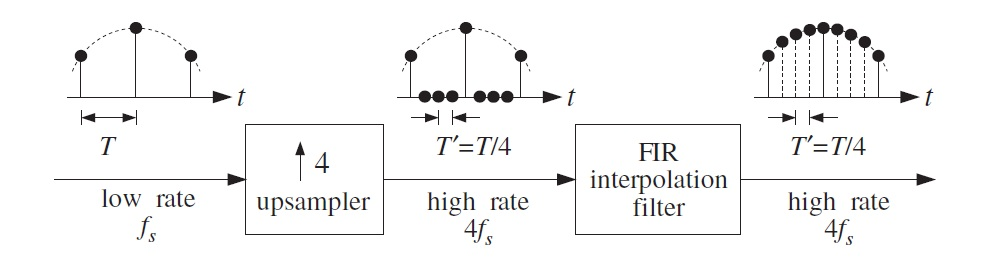
\includegraphics[width=10cm]{images/IntDecOv_IncSamplingRate.jpg}
\end{center}

There are now two discrete times, a fast one $n'$ and a slow one called $n$. 
The effect on the spectrum of a signal and the advantage in DA-Conversion is
shown in the following figure (left: original spectrum, right: spectrum
at high rate).

\begin{center}
	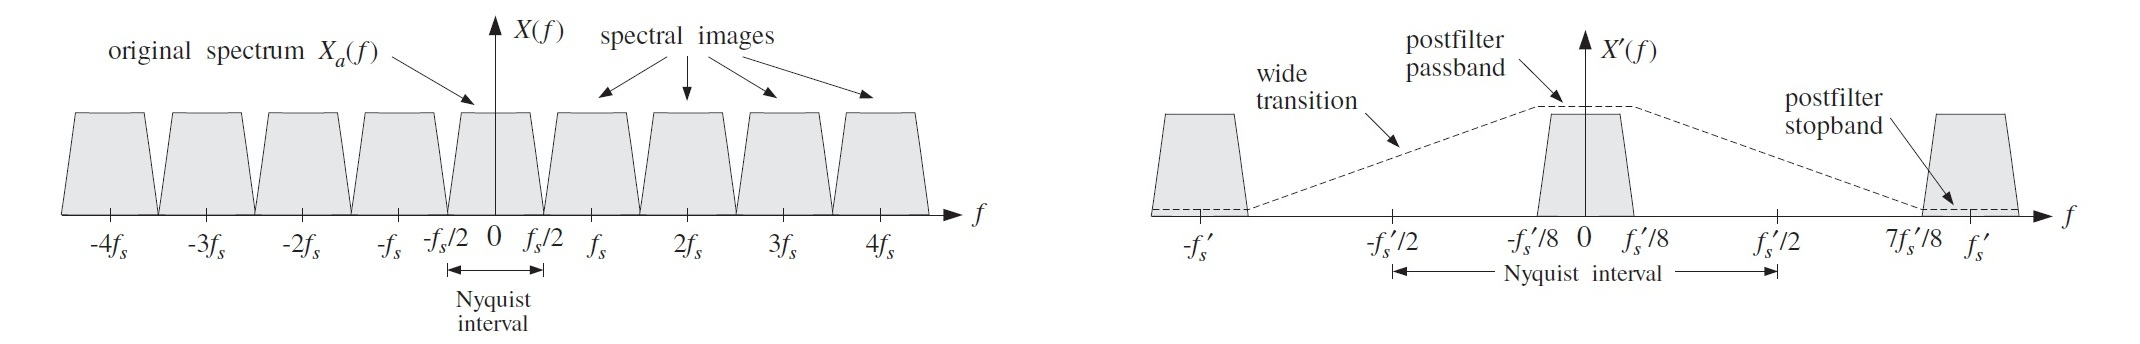
\includegraphics[width=16cm]{images/IntDecOv_Spectrum.jpg}
\end{center}

The Job of the FIR filter is to move the zeros to the appropriate values, 
or to erase the spectral copies of the original spectrum in the new 
Nyquist band. \\

\begin{center}
	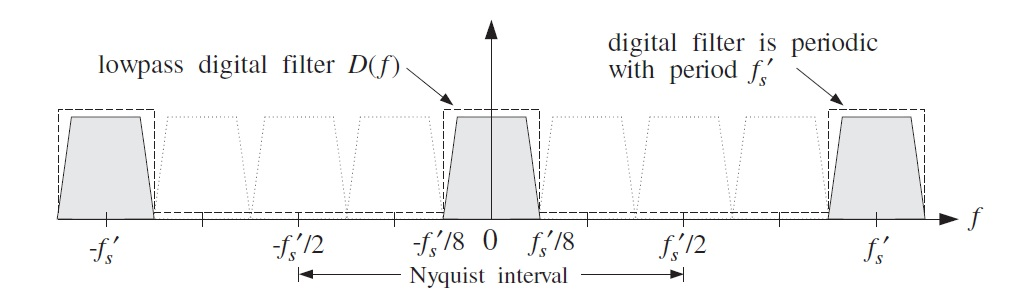
\includegraphics[width=8cm]{images/IntDecOv_Filter.jpg}
\end{center}

The ideal lowpass filter for an $L$-fold interpolation is operating at the fast
sampling rate $f'_s=L f_s$ and has its cutoff frequency at the low-sampling
rate's Nyquist frequency $f_s/2$.

\begin{equation*}
	f_c = \frac{f_s}{2}=\frac{f'_s}{2L}
	\qquad
	\omega'_c = \frac{2\pi f_c}{f'_s}=\frac{\pi}{L}
\end{equation*}

\begin{tabularx}{\linewidth}{Xl}
	FIR approximation to the ideal interpolator (non causal):
	& $d(k')=\frac{\sin(\pi k'/L)}{\pi k'/L}$, with $-LM\leq k'\leq LM$\\
	By delaying this filter by LM samples, it gets causal: 
	& $d(k')=\frac{\sin(\pi (n'-LM)/L)}{\pi (n'-LM)/L}$ \\
	Using a Hamming window: & $h(n')=w(n')d(n'-LM)$ \\
	with & $w(n') = 0.54-0.46\cos(\frac{2\pi n'}{N-1})$ \\
\end{tabularx} \\

The output of the non causal FIR interpolator filter is obtained as the
convolution of the upsampled signal with the filter 

\begin{equation*}
	y_{up}(n') = \sum\limits_{k'=-LM}^{LM}d(k')x_{up}(n'-k')
\end{equation*}


\subsubsection{Polyphase Form\buchSeite{640ff}}
%TODO: bild zeichnen, einfügen, beschriften
Suppose the low-rate time instants are $n$, then the fast-rate time instants
can be described as $n' = NL+i$ for $i=0,1,\ldots,L-1$. The output is therefore

\begin{equation*}
	y_{up}(nL+i) = \sum\limits_{k=-M}^{M-1}\sum\limits_{j=0}^{L-1} d(kL+j) x_{up}(nL+i-kL-j)
\end{equation*}

which allows us to split the output $y_{up}$ into $y_i(n)=y_{up}(nL+i)$. 
We can also define the \emph{$i$th polyphase subfilter} as

\begin{equation*}
	d_i(k) = d(kL+i) \:,\qquad -M \leq k \leq M-1 \:,\quad i=0,1,\ldots,L
\end{equation*}

The $i$th outputs can now be calculated in terms of the slow-rate samples

\begin{equation*}
	y_i(n) = \sum\limits_{k=-M}^{M-1}d_i(k) x(n-k) \:,\qquad i=0,1,\ldots,L-1
\end{equation*}

The output $y_{up}$ is now only calculated in terms of the slow sampling rate,
which decreases the computational rate in terms of multiplications per second by
a factor of $L$, from $R = NLf_s$ (direct from) to $R = Nf_s$ (polyphase form). 


\subsubsection{Frequency domain characteristics}
To discuss the interpolation in the frequency domain, we introduce the different
unit delays $z$ (low sampling rate = long delay) and $\zeta$ 
(high sampling rate = short delay)

\begin{equation*}
	z = \zeta^L \qquad \Leftrightarrow \qquad \zeta = z^{1/L}
\end{equation*}

The high-rate output can now be written in the $z$-Domain as

\begin{equation*}
	Y_{up}(\zeta) = \sum\limits_{i=0}^{L-1} \zeta^{-i} Y_i(\zeta^L)
	= \sum\limits_{i=0}^{L-1} z^{-i/L} Y_i(z)
\end{equation*}

which is what we already know from the time domain. The filter $D(\zeta)$
similarly is

\begin{equation*}
	D(\zeta) = \sum\limits_{i=0}^{L-1} \zeta^{-i} D_i(\zeta^L)
	= \sum\limits_{i=0}^{L-1} z^{-i/L} D_i(z)
\end{equation*}

The 0th polyphase subfilter $d_0(k)$ should of course return the same value as
the input $x(n)$, so the impulse response must be a dirac: 
$d_0(k) = d(kL) = \delta(k)$. \\

The ideal filter which removes all spectral copies would generally have 
the following characteristics
\begin{equation*}
	D(f) = \begin{cases}
		L\:,	& \text{if} \quad |f|\leq\frac{f_s}{2} \\
		0\:,	& \text{if} \quad \frac{f_s}{2}\leq |f|\leq\frac{f'_s}{2}
	\end{cases}
\end{equation*}

The ideal reconstructor $d(k)$, running at the higher rate $f_s'$ would
therefore be
\begin{equation*}
	d(k') = \frac{\sin(\pi k' / L)}{\pi k' / L}
\end{equation*}

This reconstructor is usually implemented using a Kaiser window design. 

\subsection{Linear and Hold Interpolators\buchSeite{657ff}}
The reconstructor described above is the ideal interpolator. Nevertheless
there exist simpler interpolators, such as the linear and the hold interpolators.
Not surprising, these are not as good as the ideal interpolator, but especially
at high sample rates, the advantage of less calculations overweights the
downsides.

\subsubsection{Hold Interpolator}
\begin{multicols}{2}
	\begin{align*}
		d(k') &= \begin{cases}
			1\:, & \text{if} \quad 0\leq k' \leq L -1\\
			0\:, & \text{otherwise}
		\end{cases} \\
		y_{up}(nL+i) &= x(n) \\
		D(f) &= \frac{\sin(\pi f/f_s)}{\sin(\pi f/Lf_s)}e^{-j\pi(L-1)f/(Lf_s)}
	\end{align*}
	
	The polyphase subfilters $d_i(k)$ will then be
	
	\begin{equation*}
		d_i(k) = \delta(k)
	\end{equation*}
	
\vfill
\columnbreak
	\begin{center}
		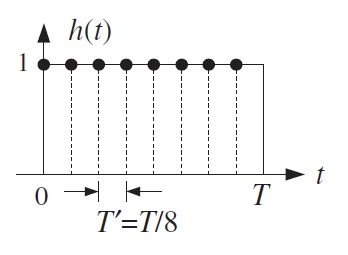
\includegraphics[width=5cm]{images/IntDecOv_Hold.jpg}
	\end{center}	
\vfill
\end{multicols}

\subsubsection{Linear Interpolator}
\begin{multicols}{2}
	\begin{align*}
		d(k') &= \begin{cases}
			1-\frac{|k'|}{L}\:, & \text{if} \quad |k'|\leq L -1\\
			0\:, & \text{otherwise}
		\end{cases} \\
		y_{up}(nL+i) &= (1-\frac{i}{L})x(n)+\frac{i}{L}x(n+1) \\
		D(f) &= \frac{1}{L}\left|\frac{\sin(\pi f/f_s)}{\sin(\pi f/Lf_s)}\right|^2
	\end{align*}
	
	The polyphase subfilters $d_i(k)$ will then be
	
	\begin{equation*}
		d_i(k) = (1-\frac{i}{L}) \delta(k) + \frac{i}{L} \delta(k+1)
	\end{equation*}	
\vfill
\columnbreak
	\begin{center}
		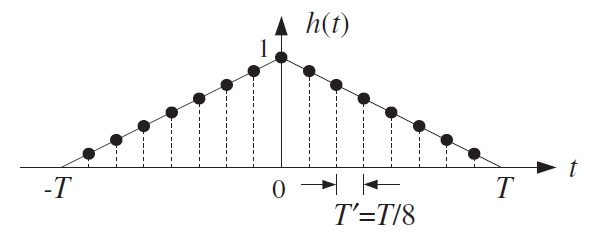
\includegraphics[width=0.8\linewidth]{images/IntDecOv_Linear.jpg}
	\end{center}
\vfill
\end{multicols}

		
\subsection{Design Examples\buchSeite{661ff}}
%TODO!!!!

\subsection{Decimation and Oversampling\buchSeite{686ff}}
Decimation is the inverse of oversampling, thus the sampling rate is reduced
from a high rate $f_s'$ to a low rate $f_s = f_s' / L$. 

\begin{center}
	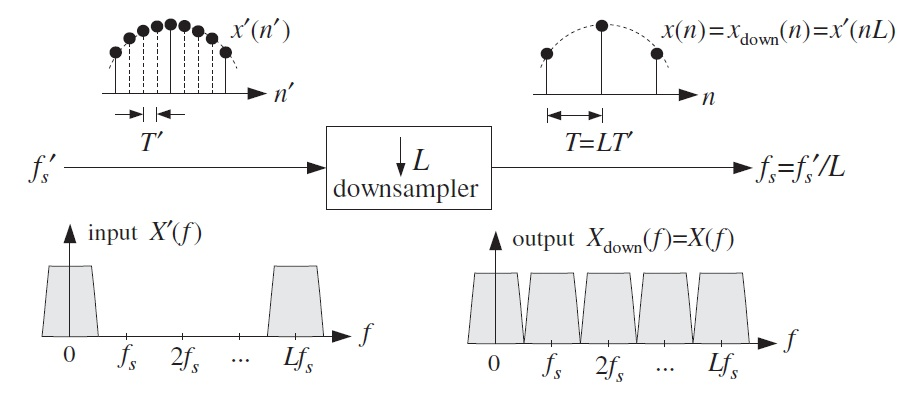
\includegraphics[width=10cm]{images/IntDecOv_Downsampler.jpg}
\end{center}

Downsampling is simply the process of discarding $L-1$ samples:

\begin{equation*}
	x_{down}(n) = \left.x'(n')\right|_{n'=nL} = x'(nL)
\end{equation*}

Caution: if the high rate spectrum occupies more than the low rate Nyquist rate
there \emph{will} be aliasing. \\

The ideal \emph{decimator} therefore contains a decimation filter, which 
operates at the high frequencies and cuts out the low rate Nyquist band.

\begin{center}
	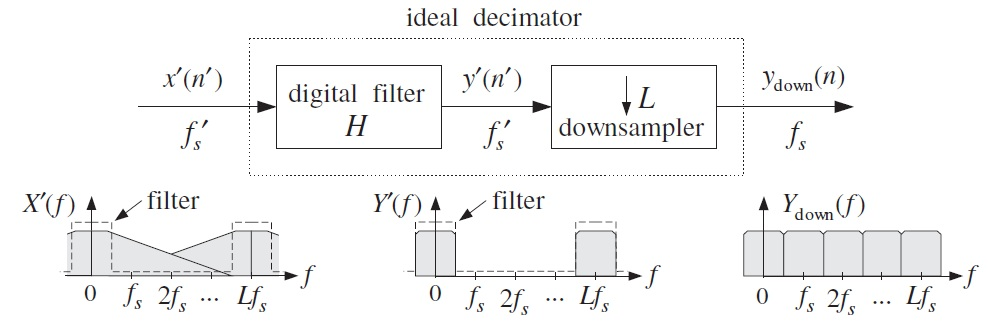
\includegraphics[width=12cm]{images/IntDecOv_Decimator.jpg}
\end{center}

The decimation filter is similar to the interpolation filter, except that
it's DC gain is unity instead of $L$. A length-$N$ FIR decimation filter
can therefore be obtained by

\begin{equation*}
	h(n') = w(n') d(n'-LM) \:,\qquad \text{where} \quad 
	d(k') = \frac{\sin(\pi k'/L)}{\pi k'}
\end{equation*}

Since only every $L$th output sample is needed, the filter output does
not need to be calculated for every fast rate sample, reducing the computational
cost by a factor $L$ to $R = \frac{1}{L} N f_s' = N f_s$. \\

%TODO bild!!!!

Multistage designs are very popular for decimation filters. The early filters will
then be fast but simple, while later filters are slow but very precise. For fast
signals, often a simple FIR averaging filter is used. The last, slowest filter
can then be designed to fix the overall frequency response.


\subsection{Noise Shaping Quantizer\buchSeite{598ff}}

\paragraph{First-order delta-sigma A/D converters}
For first order delta-sigma A/D converters, only one bit is used: $B'=1$. For
slow signals, the quantization error will be small. The system will therefore
be oversampled such that the quantization noise is moved into higher frequencies,
which are then suppressed by the digital decimation filter.

\begin{center}
	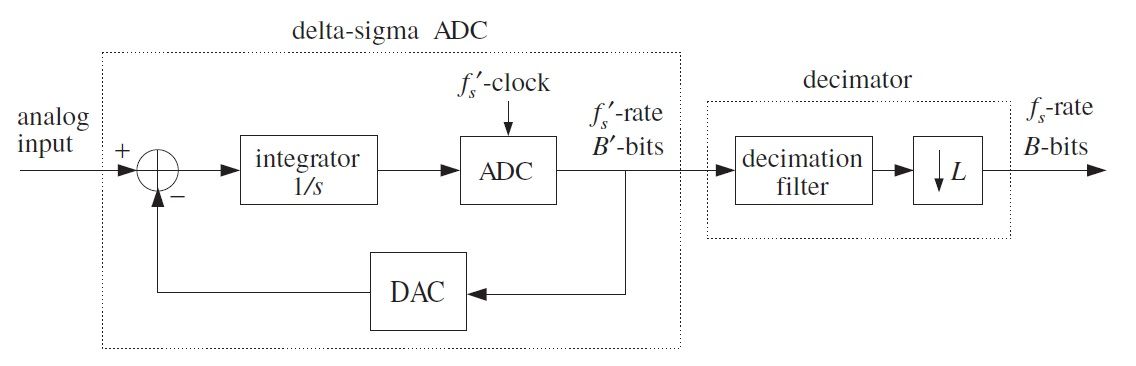
\includegraphics[width=12cm]{images/IntDecOv_SigmaDelta.jpg}
\end{center}

To be able to create a discrete time model, we replace the quantizer by
an additive quantization noise model.

\begin{center}
	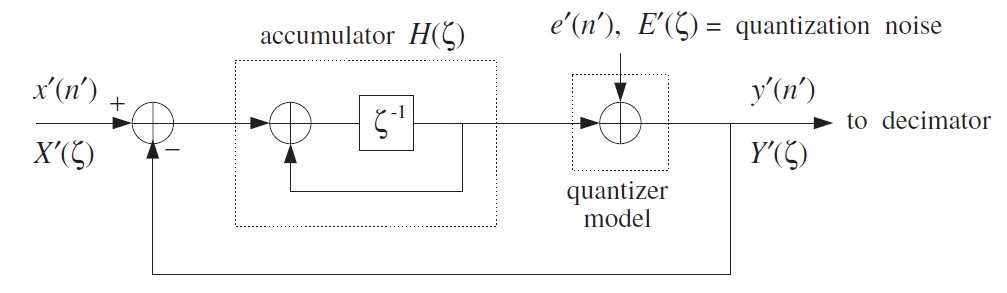
\includegraphics[width=12cm]{images/IntDecOv_SigmaDeltaModel.jpg}
\end{center}

The transfer functions for the input $X$ and the noise $NS$ will then be

\begin{equation*}
	H_X(\zeta) = \zeta^{-1} \qquad H_{NS}(\zeta) = 1 - \zeta^{-1}
\end{equation*}

or for higher orders $p$: $H_{NS}(\zeta) = (1-\zeta^{-1})^p$. \\

This leads to the known relationship of

\begin{equation*}
	\Delta B = (p+0.5) \log_2 L - 0.5 \log_2\left(\frac{\pi^{2p}}{2p+1}\right)
\end{equation*}


\paragraph{Oversampled noise shaping requantizers for D/A conversion}
Similarly, noise shaping and oversampling can be used for D/A conversion.

\begin{center}
	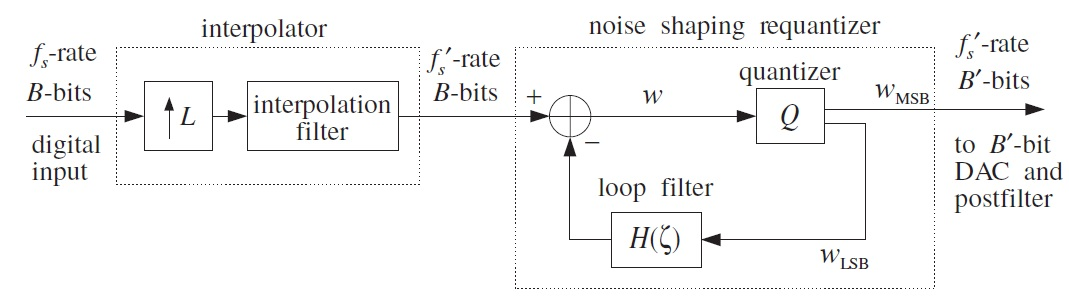
\includegraphics[width=12cm]{images/IntDecOv_Requantizer.jpg}
\end{center}

Again, using a discrete time model and a linear stochastic quantization
noise source, one gets to the following transfer functions for first-order 
or higher-order noise shaping filters

\begin{align*}
	H(\zeta) &= \zeta^{-1} \qquad &
	H_{NS}(\zeta) &= (1-\zeta^{-1}) \qquad
	& \text{first-order} \\
	H(\zeta) &= 2 \zeta^{-1} - \zeta^{-2} \qquad &
	H_{NS}(\zeta) &= (1-\zeta^{-1})^2 \qquad
	& \text{second-order}
\end{align*}

and again

\begin{equation*}
	\Delta B = (p+0.5) \log_2 L - 0.5 \log_2\left(\frac{\pi^{2p}}{2p+1}\right)
\end{equation*}